%----------------------------------------------------------------------------------------
% PACKAGES AND DOCUMENT CONFIGURATIONS
%----------------------------------------------------------------------------------------

  \documentclass[12pt]{article}

  \usepackage{hyperref}
  \usepackage{fancyhdr} % Required for custom headers
  \usepackage{lastpage} % Required to determine the last page for the footer
  \usepackage{extramarks} % Required for headers and footers
  \usepackage[usenames,dvipsnames]{color} % Required for custom colors
  \usepackage{graphicx} % Required to insert images
  \usepackage{listings} % Required for insertion of code
  \usepackage{courier} % Required for the courier font
  \usepackage{lipsum} % Used for inserting dummy 'Lorem ipsum' text into the template
  \usepackage{wrapfig}
  \usepackage{color}
  \usepackage{lscape}

  \setlength\parindent{0pt} % Removes all indentation from paragraphs
  \renewcommand{\labelenumi}{\alph{enumi}.} % Make numbering in the itemize environment by letter rather than number (e.g. section 6)

  % Margins
  \topmargin=-0.7in
  \evensidemargin=0.2in
  \oddsidemargin=-0.2in
  \textwidth=7.0in
  \textheight=9.0in
  % \headsep=0.25in

  % \linespread{1.1} % Line spacing

  \definecolor{dkgreen}{rgb}{0,0.6,0}
  \definecolor{gray}{rgb}{0.5,0.5,0.5}
  \definecolor{mauve}{rgb}{0.58,0,0.82}
  \definecolor{greyish}{rgb}{0.96,0.96,0.96}

  \lstset{
    backgroundcolor=\color{greyish},   % choose the background color; you must add \usepackage{color} or \usepackage{xcolor}
    frame=tblr,
    numbers=left,                       % where to put the line-numbers; possible values are (none, left, right)
    numbersep=5pt,                   % how far the line-numbers are from the code
    numberstyle=\tiny\color{mygray}, % the style that is used for the line-numbers
    language=Ruby,
    aboveskip=3mm,
    belowskip=3mm,
    showstringspaces=false,
    columns=flexible,
    basicstyle={\footnotesize\ttfamily},
    numbers=none,
    numberstyle=\tiny\color{gray},
    keywordstyle=\color{blue},
    commentstyle=\color{dkgreen},
    stringstyle=\color{mauve},
    breaklines=true,
    breakatwhitespace=true
    tabsize=3
  }

  \begin{document}
  \begin{titlepage}

%----------------------------------------------------------------------------------------
% TITLE PAGE INFORMATION
%----------------------------------------------------------------------------------------
 \newcommand{\HRule}{\rule{\linewidth}{0.5mm}} % Defines a new command for the horizontal lines, change thickness here
  \begin{center} % Center everything on the page

  %----------------------------------------------------------------------------------------
  % HEADING SECTIONS
  %----------------------------------------------------------------------------------------
  \textsc{\large Faculty of Computers, Informatics and Microelectronics}\\[0.5cm]
  \textsc{\large Technical University of Moldova}\\[1.2cm] % Name of your university/college
  \vspace{35 mm}
  \textsc{\Large PAD}\\[0.5cm] % Major heading such as course name
  %\textsc{\large Laboratory work \#1-3}\\[0.5cm] % Minor heading such as course title
  \textsc{\large Laboratory work \# 1}\\[0.5cm] % Minor heading such as course title

  %----------------------------------------------------------------------------------------
  % TITLE SECTION
  %----------------------------------------------------------------------------------------
  \vspace{10 mm}
  \HRule \\[0.4cm]
  { \LARGE \bfseries GIT: source code distributed systems. }\\[0.4cm] % Title of your document
  \HRule \\[1.5cm]

  %----------------------------------------------------------------------------------------
  % AUTHOR SECTION
  %----------------------------------------------------------------------------------------
      \vspace{35mm}

      \begin{minipage}{0.4\textwidth}
      \begin{flushleft} \large
      \emph{Author:}\\
      Petru \textsc{Negrei} % Your name
      \end{flushleft}
      \end{minipage}
      ~
      \begin{minipage}{0.4\textwidth}
      \begin{flushright} \large
      \emph{Supervisor:} \\
      D. \textsc{Ciorba} % Supervisor's Name
      \end{flushright}
      \end{minipage}\\[4cm]

      \vspace{5 mm}
      % If you don't want a supervisor, uncomment the two lines below and remove the section above
      %\Large \emph{Author:}\\
      %John \textsc{Smith}\\[3cm] % Your name

      %----------------------------------------------------------------------------------------
      % DATE SECTION
      %----------------------------------------------------------------------------------------

      {\large September 2014}\\[3cm] % Date, change the \today to a set date if you want to be precise

      %----------------------------------------------------------------------------------------
      % LOGO SECTION
      %----------------------------------------------------------------------------------------

      %\includegraphics{Logo}\\[1cm] % Include a department/university logo - this will require the graphicx package

      %----------------------------------------------------------------------------------------

      \vfill % Fill the rest of the page with whitespace
      \end{center}
      \end{titlepage}

      % \newpage
      % \tableofcontents
      % \newpage

%----------------------------------------------------------------------------------------
% Introduction
%----------------------------------------------------------------------------------------

  \section{Introduction}

  \subsection{Topic}

  Git: Distributed revision control systems.

  \subsection{Objective}

  To work with Git tools and study its possibilities.

  \subsection{Generic requirements}

  \subsubsection{Task}

  \begin{itemize}
    \item Initialise a local git repository;
    \item Create and link with repository from Git Lab account;
    \item Create 3 branches. On each branch commit 3 modifications. Push the local
              modifications to the remote repository.
  \end{itemize}

  \subsubsection{Report}

  Report will containt a short description of work done, and will present necesary information
  about tools, algorithms used or studied.

%----------------------------------------------------------------------------------------
% Implementation
%----------------------------------------------------------------------------------------

  \section{Implementation}

    \subsection{Installation}
    It is easiest to install Git on Linux using the preferred package manager of your Linux distribution.
    On Debian/Ubuntu.

    \begin{lstlisting}
      $ apt-get install git
    \end{lstlisting}

    \subsection{Configuration}

    The first thing you should do after you install Git is to set your user name and e-mail address.
    This is important because every Git commit uses this information, and it’s immutably baked into
    the commits you pass around.

    \begin{itemize}
      \item \textbf{Username:} First you need to tell git your name, so that it can properly label the commits you make.
      \item \textbf{Email:}  Git saves your email address into the commits you make. We use the email address to associate your commits with your GitHub or other account.
    \end{itemize}

    \begin{lstlisting}
     git config --global user.name "Your Name Here"
     git config --global user.email "your_email@youremail.com"
    \end{lstlisting}

  \subsection{Initialize an empty repository}

    Go to the project’s directory and type the below commands this will initialize
    the repository to git :

    \begin{lstlisting}
        git init
        git add .
        touch README.md
        git commit -m "initial commit"
    \end{lstlisting}

  \subsection{Link local and remote repositories}

    Before you can send your changes of the project to the remote repository
    you need to link your local with the remote one. There are 2 ways to connect
    with the GitLab repository: HTTPS or SSH. I used the SSH method to establish
    a connection. \\

    The keys are situated in the `~/.ssh' directory, first you need to verify if there are
    already generated keys.

    \begin{lstlisting}
        # check id_rsa.pub file
        $ ls ~/.ssh | grep id_rsa.pub
    \end{lstlisting}

    If the file doesn't exist then we need to generate a new SSH key, by typing the
    command below. After the new key is generated you need to link to your GitLab account,
    located under `Profile settings`, `SSH Keys`.

    \begin{lstlisting}
        # generate rsa key
        $ ssh-keygen -t rsa -C "you_email@example.com"
        # verify if the account was linked
        $ ssh -T @git@gitlab.ati.utm.md
    \end{lstlisting}

    \subsection{Remote repository}

    The next step is to create a git repository on you GitLab account, named \textit{lab}. Then I linked
    it with my local repository by typing the following command: \\

    \begin{lstlisting}
      $ git remote add origin git@gitlab.ati.utm.md:petru.negrei/lab.git
    \end{lstlisting}

    When you need to share your code you need to push your branch to a your remote repository.
    Your local branches aren’t automatically synchronized to the remotes you write to — you have to explicitly push the branches you want to share. \\ \\

    And the last step is to push to the remote repository.  Now your code is on remote repository, and can be seen by everyone colaborating with you.

    \begin{lstlisting}
      $ git push origin master
    \end{lstlisting}

    \subsection{Working with branches}

    Here I will explain the workflow of laboratory most important part. I tried to emulate the work made during a real project. \\

    First thing I did was to use \textit{tags}, in order to tag specific points in history as being important.
    Generally, people use this functionality to mark release points (v1.0, and so on), so I started by tagging \textit{master 0.1}. \\

    Next step I added some commit on \textbf{master} branch and then I created a new branch named \textbf{develop}. Ussually
    \textbf{develop} branch is were all work is done. Here I added some commits refering to \textit{improvements} added to the project. \\

    Next I created another branch named \textbf{feature}, this branch purpose is to contain work done relating to new feature that will
    be added to the project, here also I added some commits, and then merged \textit{feature} and \textit{develop} branches. \\

    Next I created another branch named \textbf{release}, this branch purpose is to prepare the project for release, and to fix existing
    bugs and add last touches to the current version of the project. After couple commit I merged the \textit{feature} branch and
    \textit{master} branch, adding a new tag \textit{v1.0}. \\

    You can see the current state of the project in the figure below. \\ \\

    \begin{minipage}[b]{1.0\linewidth}
      \begin{center}
        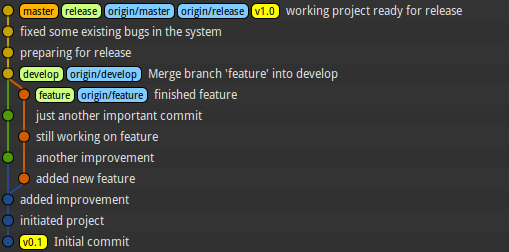
\includegraphics[width=0.7\textwidth]{work}
         \\ Fig. 1 History
      \end{center}
    \end{minipage}

    \newpage

    Below I will list some of the commands used during the implementation of the given task:

    \begin{itemize}
      \item \textit{git status} - check the current state of the repository, showing the untracked (created files),
      modified of staged files.
      \item \textit{git checkout -b "branch name"} - command used to create branches.
      \item \textit{git checkout "branch name"} - command used in order to switch between branches.
      \item \textit{git merge "branch name"} - merges the current branch with the "branch name".
      \item \textit{git push and pull} - commands used to check for changes or to update your changes to the
      remote repository.
    \end{itemize}

  \section{Conclussion}

  I previously worked with Git, which is a great Distributed Version Control System that fully mirror the repository.
  That allow the posibility to copy the back up from any client ( that has this repo ),  to the server, in case the server is down,
  and need to be restored.\\

  Distributed revision control systems takes a peer-to-peer approach to version control, as opposed to centralized system.
  Rather than a single, central repository (usually server), each peer has a working copy of the codebase as a coplete repository.
  Distributed revision control synchronizes repositories by exchanging data (sets of changes) between peers. Some of the important
  benefits of distributed systems are:
  \textit{
  \begin{itemize}
    \renewcommand{\labelitemi}{$\circ$}
    \item Common operations (such as commits, viewing history, and reverting changes) are fast, because there is no need to communicate with a central server.
    \item Communication is only necessary when sharing changes among other peers.
    \item Each working copy effectively functions as a remote backup of the codebase and of its change-history, protecting against data loss.
  \end{itemize}
}
  Thus with the help of Git and Github (which is a repository web-based hosting service),
  we can have several remote repositories that can work on different machine with different users, that can collaborate with
  each other, in different ways simultaneosly within the same project. \\

  \textbf{Link to Repository: } \url{https://gitlab.ati.utm.md/petru.negrei/lab}

   \section{References}

   \begin{itemize}
      \item Scott Chacon, Pro Git, July 29, 2009 \url{http://git-scm.com/book}
      \item Git How To,  \url{http://githowto.com/}
      \item Atlassian, Git Tutorials,  \url{https://www.atlassian.com/git/tutorial}
      \item Vincent Driessen, A successful Git branching model, January 05, 2010,  \url{http://nvie.com/posts/a-successful-git-branching-model/}
      \item Code School, Try Git, Free course,  \url{https://www.codeschool.com/courses/try-git}
      \item  Code School, Git Real, Free preview,  \url{https://www.codeschool.com/courses/git-real}
      \item Code School, Git Real 2, Free preview,  \url{https://www.codeschool.com/courses/git-real-2}
      \item Linux.conf.au 2013 - Git For Ages 4 And Up, Youtube,  \url{https://www.youtube.com/watch?v=1ffBJ4sVUb4}
   \end{itemize}

\end{document}

